\documentclass[english,serif,mathserif,xcolor=pdftex,dvipsnames,table]{beamer}
\usetheme[informal]{gc3}
\usepackage{gc3}

\title[OOP 2]{%
  Object-oriented programming, II
}
\author[GC3]{%
  GC3: Grid Computing Competence Center, \\
  University of Zurich
}
\date{Mar.~19--20, 2014}

\begin{document}

% title frame
\maketitle


\begin{frame}
  \frametitle{What we shall see in this part}

  How to use Object-oriented programming for effective code reuse.

  \+
  We shall use mainly
  \href{http://mathworld.wolfram.com/ComplexNumber.html}{complex
    numbers} as examples.
\end{frame}


\begin{frame}
  \frametitle{Recall: \emph{What is a complex number?}}

  \begin{columns}
    \begin{column}{0.6\linewidth}
      \raggedleft
      A complex number $\mathbf{z}$ has the form $\mathbf{z} = z_1 + z_2i$, where \\
      $z_1$ and $z_2$ are real numbers; \\
      $z_1$ is called the real part \\
      and $z_2$ the imaginary part.
    \end{column}
    \begin{column}{0.4\linewidth}
      \centering
      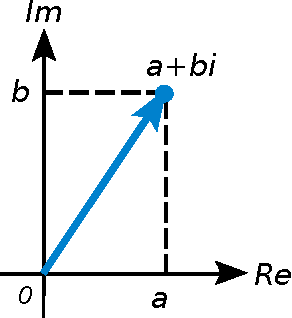
\includegraphics[height=5\baselineskip]{fig/ComplexNumber}
    \end{column}
  \end{columns}

  \+
  The set of complex numbers is a field with the two operations:
  \begin{itemize}
  \item
    \emph{addition:} if $\mathbf{z} = \mathbf{x} + \mathbf{y}$,
    then:
    \begin{gather*}
      z_1 = x_1 + y_1, \quad \text{and} \quad z_2 = x_2 + y_2.
    \end{gather*}

  \item
    \emph{multiplication:} if $\mathbf{z} = \mathbf{x} \cdot
    \mathbf{y}$, then:
    \begin{gather*}
      z_1 = x_1\cdot y_1 - x_2 \cdot y_2,
      \quad\text{and}\quad
      z_2 = x_2\cdot y_1 + x_1\cdot y_2.
    \end{gather*}

  \end{itemize}

  \begin{references}
    Images courtesy of \href{http://en.wikipedia.org/wiki/Complex_number}{Wikipedia}.
  \end{references}
\end{frame}


\begin{frame}[fragile]
  \frametitle{Naive complex numbers in Python}
  \begin{columns}[t]
    \begin{column}{0.5\textwidth}
\begin{lstlisting}[showstringspaces=false]
class ComplexNum(object):
  "A complex number z = z1 + z2*i."
  def __init__(self, z1, z2):
    self.re = z1
    self.im = z2
  def __add__(self, other):
    return ComplexNum(
      self.re+other.re, self.im+other.im)
  def __mul__(self, other):
    return ComplexNum(
      self.re*other.re - self.im*other.im,
      self.re*other.im + self.im*other.re)
  def __str__(self):
    return ("%g + %gi" % (self.re, self.im))
  def __eq__(self, other):
    return (self.re == other.re) \
           and (self.im == other.im)
\end{lstlisting}
    \end{column}
    \begin{column}{0.5\textwidth}
      \raggedleft
      This code defines a Python object that implements a complex number.
    \end{column}
  \end{columns}

  \+
  {\scriptsize Source code available at:
    \url{https://raw.github.com/gc3-uzh-ch/python-course/master/complexnum.py}}
\end{frame}


\begin{frame}[fragile]
  \frametitle{What does \texttt{ComplexNum} do?}
  \begin{columns}
    \begin{column}[t]{0.5\linewidth}
      We can create complex numbers by initializing them with the real
      and imaginary part:
\begin{lstlisting}
>>> u = ComplexNum(1,0)
>>> i = ComplexNum(0,1)
>>> z = ComplexNum(1,1)
\end{lstlisting}
    \end{column}
    \begin{column}[t]{0.5\linewidth}
      The \lstinline|__str__| method provides the familiar
      representation:
\begin{lstlisting}
>>> print(u)
1 + 0i
>>> print(i)
0 + 1i
>>> print(z)
1 + 1i
\end{lstlisting}
    \end{column}
  \end{columns}

  \+
  \begin{columns}
    \begin{column}[t]{0.5\linewidth}
      The \lstinline|__add__| method makes the ``\texttt{+}'' operator work:
\begin{lstlisting}
>>> w = u + i
>>> print(w)
1 + 1i
\end{lstlisting}
    \end{column}
    \begin{column}[t]{0.5\linewidth}
      The \lstinline|__mul__| method makes the ``\texttt{*}'' operator work:
\begin{lstlisting}
>>> m = i*i
>>> print(m)
-1 + 0i
\end{lstlisting}
    \end{column}
  \end{columns}
\end{frame}


\begin{frame}[fragile]
  \begin{exercise}
    Add a \lstinline|to_power| method to class \texttt{ComplexNum},
    that takes an integer number as argument and returns the complex
    number raised to that power.

    \+
    Example:
\begin{lstlisting}
>>> z = Complex(1,1)
>>> w = z.to_power(3)
>>> print(w)
-2 + i2
\end{lstlisting}

    \+ Verify that \lstinline|z.to_power(1)|,
    \lstinline|z.to_power(2)| and \lstinline|z.to_power(3)| yield the
    same result as \lstinline|z|, \lstinline|z*z| and
    \lstinline|z*z*z|.
  \end{exercise}
\end{frame}


\begin{frame}[fragile]
  \frametitle{\texttt{Vector} vs \texttt{ComplexNum}}

  There's a lot of similarities in the two classes!

  How can we share code between the two?

  \begin{columns}[t]
    \begin{column}{0.5\textwidth}
\begin{lstlisting}[basicstyle=\tiny\ttfamily,showstringspaces=false]
class Vector(object):

  ~\HL[Yellow!25]{\textbf{def} {\color{Red}\bfseries \_\_init\_\_}(\textbf{self}, x, y):}~
    self.x = x
    self.y = y

  ~\HL[Yellow!25]{\textbf{def} {\color{Red}\bfseries \_\_eq\_\_}(\textbf{self}, other):}~
    return (self.x == other.x) \
            and (self.y == other.y)

  ~\HL[Yellow!25]{\textbf{def} {\color{Red}\bfseries \_\_add\_\_}(\textbf{self}, other):}~
    return Vector(
      self.x+other.x, self.y+other.y)

  def __mul__(self, scalar):
    return Vector(
      scalar*self.x,
      scalar*self.y)

  def __str__(self):
    return ("<%g,%g>" % (self.x, self.y))
\end{lstlisting}
    \end{column}
    \begin{column}{0.5\textwidth}
\begin{lstlisting}[basicstyle=\tiny\ttfamily,showstringspaces=false]
class ComplexNum(object):

  ~\HL[Yellow!25]{\textbf{def} {\color{Red}\bfseries \_\_init\_\_}(\textbf{self}, z1, z2):}~
    self.re = z1
    self.im = z2

  ~\HL[Yellow!25]{\textbf{def} {\color{Red}\bfseries \_\_eq\_\_}(\textbf{self}, other):}~
    return (self.re == other.re) \
           and (self.im == other.im)

  ~\HL[Yellow!25]{\textbf{def} {\color{Red}\bfseries \_\_add\_\_}(\textbf{self}, other):}~
    return ComplexNum(
      self.re+other.re, self.im+other.im)

  def __mul__(self, other):
    return ComplexNum(
      self.re*other.re - self.im*other.im,
      self.re*other.im + self.im*other.re)

  def __str__(self):
    return ("%g + %gi" % (self.re, self.im))
\end{lstlisting}
    \end{column}
  \end{columns}
\end{frame}


\begin{frame}
  \frametitle{\emph{Vectors} and \emph{Complex Numbers}}

  \begin{columns}
    \begin{column}{0.6\linewidth}
      \raggedleft
      Complex Numbers are in $1-1$ correspondence with
      points in the real plane $\mathbb{R}^2$: the set $\mathbb{C}$ of
      Complex Numbers is the set of real \emph{2D} vectors.
    \end{column}
    \begin{column}{0.4\linewidth}
      \centering
      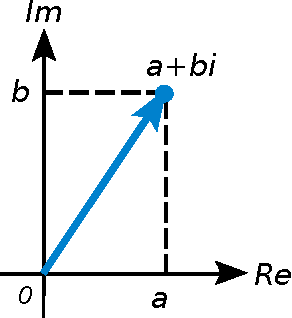
\includegraphics[height=7\baselineskip]{fig/ComplexNumber}
    \end{column}
  \end{columns}

  \+
  So we can define the class of Complex Numbers as the class of
  Vectors augmented with a multiplication operation.

  \+
  So: a Complex Number is a Vector plus some behavior.
\end{frame}


\begin{frame}[fragile]
  \frametitle{Inheritance, I}

  \begin{columns}[t]
    \begin{column}{0.5\textwidth}
\begin{lstlisting}[basicstyle=\tiny\ttfamily,showstringspaces=false]
class Vector(object):

  def __init__(self, x, y):
    self.x = x
    self.y = y

  def __eq__(self, other):
    return (self.x == other.x) \
            and (self.y == other.y)

  def __add__(self, other):
    return self.__class__(
      self.x+other.x, self.y+other.y)

  def __mul__(self, scalar):
    return Vector(
      scalar*self.x,
      scalar*self.y)

  def __str__(self):
    return ("<%g,%g>" % (self.x, self.y))
\end{lstlisting}
    \end{column}
    \begin{column}{0.5\textwidth}
\begin{lstlisting}[basicstyle=\tiny\ttfamily,showstringspaces=false]
class ~\HL{ComplexNum(Vector)}~:

  def __mul__(self, other):
    return ComplexNum(
      self.x*other.x - self.y*other.y,
      self.x*other.y + self.y*other.x)

  def __str__(self):
    return ("%g + %gi" % (self.x, self.y))
\end{lstlisting}

      \+
      This syntax means that class \texttt{ComplexNum} is a
      \emph{child}/\emph{descendant}/\emph{subclass} of class \texttt{Vector}.

      \+
      Class \texttt{Vector} is a
      \emph{parent}/\emph{ancestor}/\emph{superclass} of class
      \texttt{ComplexNum}.
    \end{column}
  \end{columns}

  \+
  {\scriptsize Source code available at:
    \url{https://raw.github.com/gc3-uzh-ch/python-course/master/vector_and_complexnum.py}}
\end{frame}


\begin{frame}[fragile]
  \frametitle{Inheritance, II}

  \begin{columns}[t]
    \begin{column}{0.5\textwidth}
\begin{lstlisting}[basicstyle=\tiny\ttfamily,showstringspaces=false]
class Vector(object):

  ~\HL{\textbf{def} {\color{Red}\bfseries \_\_init\_\_}(\textbf{self}, x, y):}~
    self.x = x
    self.y = y

  ~\HL{\textbf{def} {\color{Red}\bfseries \_\_eq\_\_}(\textbf{self}, other):}~
    return (self.x == other.x) \
            and (self.y == other.y)

  ~\HL{\textbf{def} {\color{Red}\bfseries \_\_add\_\_}(\textbf{self}, other):}~
    return self.__class__(
      self.x+other.x, self.y+other.y)

  def __mul__(self, scalar):
    return Vector(
      scalar*self.x,
      scalar*self.y)

  def __str__(self):
    return ("<%g,%g>" % (self.x, self.y))
\end{lstlisting}
    \end{column}
    \begin{column}{0.5\textwidth}
\begin{lstlisting}[basicstyle=\tiny\ttfamily,showstringspaces=false]
class ComplexNum(Vector):

  def __mul__(self, other):
    return ComplexNum(
      self.x*other.x - self.y*other.y,
      self.x*other.y + self.y*other.x)

  def __str__(self):
    return ("%g + %gi" % (self.x, self.y))
\end{lstlisting}

      \+
  All methods defined in class \texttt{Vector} are automatically
  defined \emph{(inherited)} in class \texttt{ComplexNum}.
    \end{column}
  \end{columns}
\end{frame}


\begin{frame}[fragile]
  \frametitle{Inheritance, III}

  \begin{columns}[t]
    \begin{column}{0.5\textwidth}
\begin{lstlisting}[basicstyle=\tiny\ttfamily,showstringspaces=false]
class Vector(object):

  def __init__(self, x, y):
    self.x = x
    self.y = y

  def __eq__(self, other):
    return (self.x == other.x) \
            and (self.y == other.y)

  def __add__(self, other):
    return self.__class__(
      self.x+other.x, self.y+other.y)

  ~\HL[Yellow!25]{\textbf{def} {\color{Red}\_\_mul\_\_}(\textbf{self}, other):}~
    return Vector(
      scalar*self.x,
      scalar*self.y)

  ~\HL[Yellow!25]{\textbf{def} {\color{Red}\_\_str\_\_}(\textbf{self}):}~
    return ("<%g,%g>" % (self.x, self.y))
\end{lstlisting}
    \end{column}
    \begin{column}{0.5\textwidth}
\begin{lstlisting}[basicstyle=\tiny\ttfamily,showstringspaces=false]
class ComplexNum(Vector):

  ~\HL{\textbf{def} {\color{Red}\_\_mul\_\_}(\textbf{self}, other):}~
    return ComplexNum(
      self.x*other.x - self.y*other.y,
      self.x*other.y + self.y*other.x)

  ~\HL{\textbf{def} {\color{Red}\_\_str\_\_}(\textbf{self}):}~
    return ("%g + %gi" % (self.x, self.y))
\end{lstlisting}

      \small
      \+
      Methods \lstinline|__mul__| and \lstinline|__str__| are
      defined in both classes: instances of a class use the
      definition from that class.

      \+
      We say that \texttt{ComplexNum} \emph{overrides} those
      methods from \texttt{Vector}.
    \end{column}
  \end{columns}
\end{frame}


\begin{frame}
  What happens if a descendant class re-defines a \lstinline|__init__|
  method?

  \+ \pause{\em
    The \lstinline|__init__| in the descendant class
    \emph{overrides} the method in the ancestor class.  So
    \lstinline|__init__| of the parent class(es) will not be called.
  }
\end{frame}


\begin{frame}[fragile]
  \frametitle{Constructor chaining}
  % \begin{flushright}
  %   \footnotesize%
  %   {\em ``Explicit is better than implicit''}
  %   --- T.~Peters, \href{http://www.python.org/dev/peps/pep-0020/}{The
  %     Zen of Python}
  % \end{flushright}

    When a class is instanciated, Python only calls the first
    constructor it can find in the
    \href{http://www.python.org/download/releases/2.3/mro/}{class inheritance call-chain}.

    \+ \textbf{If you need to call a parent constructor, you need
      to do it \emph{explicitly}:}
    \begin{python}
class Application(Task):
  def __init__(self, ...):
    # do Application-specific stuff here
    Task.__init__(self, ...)
    # some more Application-specific stuff
    \end{python}

    \+
    Calling a superclass constructor is optional, and
    it can happen anywhere in the \lstinline|__init__| method body.
\end{frame}


\begin{frame}[fragile]
  \frametitle{Method chaining}

  Actually, \lstinline|__init__| is not special in this regard.

  \+ When any instance method is called, Python only calls the first
  constructor it can find in the
  \href{http://www.python.org/download/releases/2.3/mro/}{class
    inheritance call-chain}.

  \+ \textbf{You can always call a superclass method by prefixing it
    with the superclass name and explicitly writing ``\texttt{self}''
    as the first argument:}
    \begin{python}
class ComplexNum(Vector):
  # ...
  def print_as_vector(self):
    return ~\HL{Vector.\_\_str\_\_(self)}~
    \end{python}
\end{frame}


\begin{frame}[fragile]
  \frametitle{Inheritance, IV}
Take a look at this Python interaction:
\begin{lstlisting}
>>> z = ComplexNum(1,0)
>>> print(z)
1 + i0
>>> w = ComplexNum(0,1)
>>> print(w)
0 + i1
>>> u = z + w
>>> print(u)
\end{lstlisting}
\only<1>{\em  What do you think will be printed now?}
\only<2>{%
  \vspace{-1.5em}
\begin{semiverbatim}
\HL{<1,1>}
\end{semiverbatim}
{\em  This is no \texttt{ComplexNum}! What's happening here?}
}%
\end{frame}


\begin{frame}[fragile]
  \frametitle{Inheritance, V}
  The answer is in the code:
    \begin{python}
class Vector(object):
  # ...
  def __add__(self, other):
    return ~\HL{Vector}~(self.x+other.x, self.y+other.y)
    \end{python}
    \pause
    The \lstinline|Vector.__add__| method returns a new
    \lstinline|Vector| instance, even when called from a
    \lstinline|ComplexNum| !
\end{frame}


\begin{frame}[fragile]
  \frametitle{Inheritance, VI}
  Correct code:
    \begin{python}
class Vector(object):
  # ...
  def __add__(self, other):
    return ~\HL{self.\_\_class\_\_}~(self.x+other.x, self.y+other.y)
    \end{python}
    Use the class of the actual instance that's passed,
    instead of hard-coding a class name.
\end{frame}


\begin{frame}[fragile]
  \frametitle{Polymorphism, I}

  The multiplication operator ``\texttt{*}'' on instances of the
  \lstinline|Vector| class works as \emph{scalar multiplication}:
\begin{lstlisting}
>>> v = Vector(1,0)
>>> print (v * 3)
<3,0>
\end{lstlisting}

  \+
  The same operator ``\texttt{*}'' on instances of the
  \lstinline|ComplexNum| class works as \emph{complex multiplication}:
\begin{lstlisting}
>>> z = ComplexNum(1,1)
>>> w = ComplexNum(2,0)
>>> print (z * w)
2 + i2
\end{lstlisting}

  \+\small
  The ability to implement different behavior for the same
  method/operator in different classes is called \emph{polymorphism}.

\end{frame}

\begin{frame}[fragile]
  \frametitle{Polymorphism, II}

  You may observe that an integer is (in particular) a complex number,
  still we cannot multiply a \texttt{ComplexNum} instance by an
  integer number:
\begin{lstlisting}
>>> print (z * 3)
Traceback (most recent call last):
  File "<stdin>", line 1, in <module>
  File "vector_and_complexnum.py", line 20, in __mul__
    self.x*other.x - self.y*other.y,
AttributeError: 'int' object has no attribute 'x'
\end{lstlisting}

\end{frame}


\begin{frame}[fragile]
  \frametitle{Polymorphism, III}

\begin{lstlisting}
>>> print (z * 3)
Traceback (most recent call last):
  File "<stdin>", line 1, in <module>
  File "vector_and_complexnum.py", line 20, in __mul__
    self.x*~\HL{other.x}~ - self.y*~\HL{other.y}~,
AttributeError: 'int' object has no attribute 'x'
\end{lstlisting}

  \+ Our code for \lstinline|ComplexNum.__mul__| implicitly assumes
  that argument \lstinline|other| has attributes \texttt{x} and
  \texttt{y}, and integers do not!
\end{frame}


\begin{frame}[fragile]
  \frametitle{The \texttt{isinstance} function}
  The \texttt{isinstance($x$, $C$)} function returns \texttt{True} if
  object $x$ is an instance of class $C$.

  \+
  \begin{columns}
    \begin{column}{0.5\textwidth}
\begin{lstlisting}
>>> isinstance(z, ComplexNum)
True
>>> isinstance(z, Vector)
True
\end{lstlisting}
    \end{column}
    \begin{column}{0.4\textwidth}
      \raggedleft
      An instance of \texttt{ComplexNum} is also an instance of
      \texttt{Vector} by inheritance.
    \end{column}
  \end{columns}
\end{frame}


\begin{frame}[fragile]
  \frametitle{The \texttt{isinstance} function}
  The \texttt{isinstance($x$, $C$)} function returns \texttt{True} if
  object $x$ is an instance of class $C$.

  \+
  \begin{columns}
    \begin{column}{0.5\textwidth}
\begin{lstlisting}
>>> isinstance(v, Vector)
True
>>> isinstance(v, ComplexNum)
False
\end{lstlisting}
    \end{column}
    \begin{column}{0.5\textwidth}
      \raggedleft
      \emph{However,} instances of \texttt{Vector} are \emph{not}
      instances of \texttt{ComplexNum}.
    \end{column}
  \end{columns}
\end{frame}


\begin{frame}[fragile]
  \frametitle{The \texttt{isinstance} function}
  The \texttt{isinstance($x$, $C$)} function returns \texttt{True} if
  object $x$ is an instance of class $C$.

  \+
  \begin{columns}
    \begin{column}{0.5\textwidth}
\begin{lstlisting}
>>> isinstance(1, int)
True
>>> isinstance(0.5, float)
True
>>> isinstance("hi!", str)
True
\end{lstlisting}
    \end{column}
    \begin{column}{0.5\textwidth}
      \raggedleft
      Basic Python objects are instances of built-in classes.
    \end{column}
  \end{columns}
\end{frame}


\begin{frame}[fragile]
  \begin{exercise}
    Modify the \lstinline|__mul__| method of class \texttt{ComplexNum}:
    \begin{itemize}
    \item If second argument \texttt{other} is an object of class
      \texttt{int} (integer) or \texttt{float} (floating-point
      number) then return the result of scalar multiplication by that number.
    \item If second argument \texttt{other} is an object of class
      \texttt{ComplexNum}, then return the result of complex
      multiplication by that number.
    \end{itemize}
  \end{exercise}
\end{frame}


% \begin{frame}
%   \frametitle{Protocols}
%   A \emph{protocol}, in the Python jargon, is an informal
%   specification of what methods an object should implement in order to
%   be used in a certain context.

%   \+ For example, objects that implement the same methods as the
%   \texttt{file} object are called ``file-like'' and can be used in
%   stead of a real file.

%   \+
%   (This corresponds to the notion of \emph{interfaces} in other
%   programming languages, but interfaces are usually a formal language
%   construct.)
% \end{frame}


\begin{frame}[fragile]
  \frametitle{\emph{Detour:} The Iterator Protocol}

  An \emph{iterator} is an object that can be used in the
  \texttt{in}-clause of a \texttt{for \ldots in \ldots} statement.

  \+
  An object can function as an iterator iff it implements a
  \texttt{next()} method, that:
  \begin{description}
  \item[\emph{either}] returns the next value in the iteration,
  \item[\emph{or}] use \lstinline|raise StopIteration| to signal the
    end of the iteration.
  \end{description}

  \+
  An object can be iterated over with \lstinline|for| if it implements a
  \lstinline|__iter__()| method that returns an iterator.

  \begin{references}
    \url{http://www.python.org/dev/peps/pep-0234/}
  \end{references}
\end{frame}


\begin{frame}[fragile]
  \frametitle{Examples of Iterators, I}

  The \texttt{file} object:
\begin{lstlisting}
>>> fd = open('welcome.py', 'r')
>>> dir(fd)
['__class__', ~\ldots,~ 'name',
 'newlines', ~\HL{\tt 'next'}~, 'read',
 ~\ldots,~  'writelines', 'xreadlines']
\end{lstlisting}

  \+
  The \texttt{.next()} method of \texttt{file} objects returns the
  lines one by one:
\begin{lstlisting}
>>> fd.next()
'#! /usr/bin/env python\n'
>>> fd.next()
'\n'
>>> fd.next()
'print ("Welcome to Python!")\n'
\end{lstlisting}

\end{frame}


\begin{frame}[fragile]
  \frametitle{Examples of Iterators, II}

  You can get an iterator from any sequence with the \texttt{iter()} built-in function:
\begin{lstlisting}
>>> S = "Python"
>>> it = iter(S)
\end{lstlisting}

  \+
  The \texttt{.next()} method of such iterators returns the
  elements of the sequence one by one:
\begin{lstlisting}
>>> it.next()
'P'
>>> it.next()
'y'
\end{lstlisting}
\end{frame}


\begin{frame}[fragile]
  \frametitle{A user-defined iterator}
  \begin{columns}[t]
    \begin{column}{0.5\textwidth}
\begin{lstlisting}
class Evens(object):

  def __init__(self, numbers):
    self._numbers = numbers

  def next(self):
      result = self._numbers.pop(0)
      while (result % 2) != 0:
          result = self._numbers.pop(0)
      return result

  def __iter__(self):
      return self
\end{lstlisting}
    \end{column}
    \begin{column}{0.5\textwidth}
      \raggedleft
      Iterate over the even numbers in a sequence.
    \end{column}
  \end{columns}

  \+
  {\scriptsize Source code available at:
    \url{https://raw.github.com/gc3-uzh-ch/python-course/master/evens.py}}
\end{frame}


\begin{frame}[fragile]
  \frametitle{Example using \texttt{Evens}, I}
\begin{lstlisting}
>>> from evens import Evens
>>> e = Evens([1,2,3,5,7,8])
>>> e.next()
2
>>> e.next()
8
>>> e.next()
Traceback (most recent call last):
  File "<stdin>", line 1, in <module>
  File "evens.py", line 12, in next
    result = self._numbers.next()
StopIteration
\end{lstlisting}
\end{frame}


\begin{frame}[fragile]
  \frametitle{Example using \texttt{Evens}, II}
\begin{lstlisting}
>>> from evens import Evens
>>> e = Evens([1,2,3,5,7,8])
>>> for num in e:
...   print num
...
2
8
\end{lstlisting}
\end{frame}


\begin{frame}[fragile]
  \begin{exercise}\small
    Define a \texttt{ReadPairs} class, with the following features.

    \+ A \texttt{ReadPairs} instance is created by passing a filename:
\begin{lstlisting}
>>> rt = ReadPairs('wt.csv')
\end{lstlisting}

    \+ Each time the \texttt{next()} method is called on a \texttt{ReadPairs} instance:
    \begin{enumerate}
    \item a line is read from the file passed to the constructor,
    \item that line is split at commas yielding two values,
    \item a 2-tuple consisting of the two values converted to integers is returned.
    \end{enumerate}

    \+ If a line is malformed (e.g., it does not contain exactly two
    values), then that line is ignored and \texttt{next()} should
    proceed to the next line.
  \end{exercise}
\end{frame}


\begin{frame}
  \frametitle{Detour: Regular Expression objects}
  The \texttt{re} module in the standard library provides
  \emph{regular expression searching}, allowing you to match a string
  against a pattern.

  \+
  \begin{describe}{re.search(pattern, string)}
    If \texttt{pattern} is matched anywhere in \texttt{string}, return
    a \emph{match object}.  Otherwise, return \texttt{None}.
  \end{describe}

  \+
  \begin{describe}{\emph{match}.group(0)}
    The entire string matched by \texttt{pattern} in a search operation.
  \end{describe}

  \+
  \begin{references}
    \url{http://docs.python.org/library/re.html}
  \end{references}
\end{frame}


\begin{frame}[fragile]
  \begin{exercise}
    Define a \texttt{Grep} iterator:
    \begin{itemize}
    \item a \texttt{Grep} instance is constructed by giving a file name and a regular expression pattern, e.g., \lstinline|g = Grep(filename, pattern)|
    \item Each call to the \texttt{next()} method returns the next line in the file that matches the regular expression \texttt{pattern}.
    \end{itemize}

    Use the \texttt{next()} method of file objects!
  \end{exercise}

  \+
  \begin{exercise}
    Define a \texttt{GrepOnlyMatching} class, similar to \texttt{Grep}
    except that its \texttt{next()} method returns only the part of
    the line that matched the \texttt{pattern} expression.
  \end{exercise}

  \+
  \begin{exercise}
    Define a \texttt{GrepExactly} class, similar to \texttt{Grep}
    except that \texttt{pattern} is now a fixed string, and the
    \texttt{next()} method returns lines that \emph{contain} it.
  \end{exercise}
\end{frame}


\begin{frame}[fragile]
  \frametitle{The ``Template method'' pattern}
\begin{lstlisting}
class Grep(object):

    def __init__(self, filename, pattern):
        self._file = open(filename, 'r')
        self._pattern = pattern

    def match(self, line):
        return re.search(self._pattern, line)

    def result(self, match, line):
        return line

    def next(self):
        line = self._file.next()
        match = self.match(line)
        while not match:
            line = self._file.next()
            match = self.match(line)
        return self.result(match, line)
\end{lstlisting}
\end{frame}


\begin{frame}[fragile]
  \frametitle{The ``Template method'' pattern, I}
  \begin{columns}[t]
    \begin{column}{0.5\textwidth}
\begin{lstlisting}
class Grep(object):

  # parts omitted

  def next(self):
    line = self._file.next()
    match = ~\HL{self.match}~(line)
    while not match:
        line = self._file.next()
        match = ~\HL{self.match}~(line)
    return ~\HL{self.result}~(match, line)
\end{lstlisting}
    \end{column}
    \begin{column}{0.5\textwidth}
      \raggedleft
      These calls delegate the actual matching and
      extraction of the result from the line to instance methods.
    \end{column}
  \end{columns}
\end{frame}


\begin{frame}[fragile]
  \frametitle{The ``Template method'' pattern, II}
  \begin{columns}[t]
    \begin{column}{0.5\textwidth}
\begin{lstlisting}

class GrepOnlyMatching(Grep):
  ~\HL{\textbf{def} result}~(self, match, line):
    return match.group(0)

class GrepExactly(Grep):
  ~\HL{\textbf{def} match}~(self, line):
    return (self._pattern in line)
\end{lstlisting}
    \end{column}
    \begin{column}{0.5\textwidth}
      \raggedleft
      So we need only re-define those methods in derived
      classes to implement a variant behavior.
    \end{column}
  \end{columns}
\end{frame}


\end{document}

%%% Local Variables:
%%% mode: latex
%%% TeX-master: t
%%% End:
